\section{Tyrimo rezultatai}
\label{sec:tyrimo_rezultatai}

Šiame skyriuje pateikiami visų atliktų tyrimų rezultatai.
\vspace{10pt}

Žymėjimai grafikuose:
\begin{itemize}
    \item „\texttt{lr}“ žymi mokymosi greitį (angl. \textit{learning rate}).
    \item „\textit{Batch GD}“ žymi paketinį gradientinį nusileidimą.
    \item „\textit{Stochastic GD}“ žymi stochastinį gradientinį nusileidimą.
    \item „\textit{Train}“ žymi mokymo duomenis.
    \item „\textit{Val}“ žymi validavimo duomenis.
    \item „\textit{Test}“ žymi testavimo duomenis.
\end{itemize}

\subsection{Paklaidos priklausomybė nuo epochų}
\label{subsec:paklaidos_priklausomybe_nuo_epochu}

Šiame poskyryje aptariama paklaidos priklausomybė nuo epochų abiems taikytiems metodams.

\subsubsection{Paketinis gradientinis nusileidimas}
\label{subsubsec:paklaidos_priklausomybe_paketinis_gradientinis_nusileidimas}

Naudojant paketinį gradientinį nusileidimą su mokymosi greičiu $\eta = 0{,}5$ ir $500$ epochų, paklaida tolygiai mažėja per visą mokymo procesą (žr.~\ref{fig:error_bgd} pav.). Galutinė mokymo paklaida – $0{,}0354$, validavimo – $0{,}0296$. Validavimo paklaida yra mažesnė nei mokymo, o tai rodo, kad modelis nėra persimokęs.

\begin{figure}[H]
    \centering
    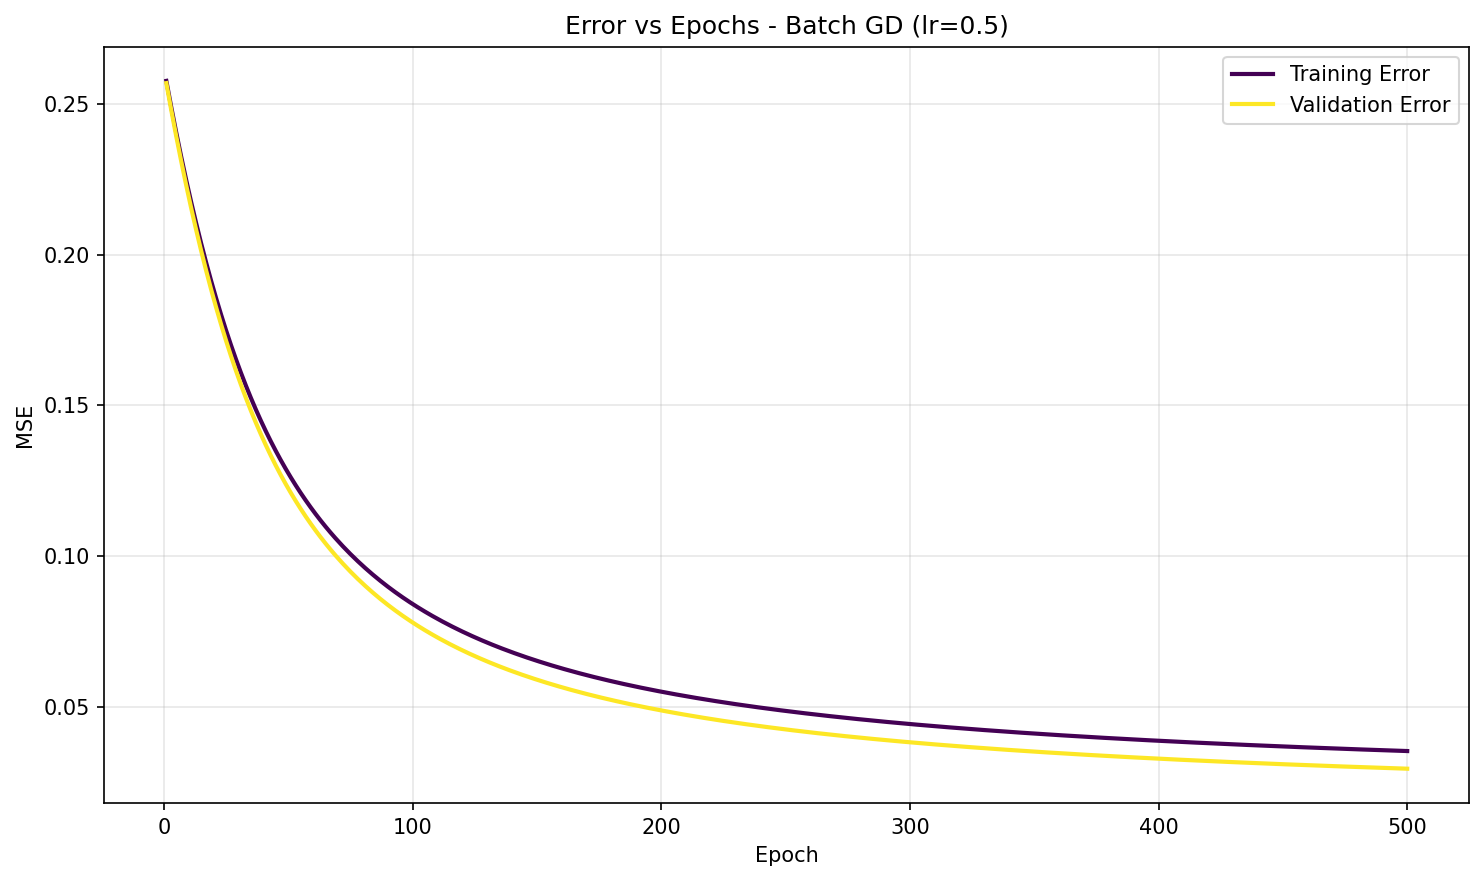
\includegraphics[width=0.85\linewidth]{2Lab/visualizations/error_bgd.png}
    \caption{Paklaidos priklausomybė nuo epochų (paketinis GN, $\eta = 0{,}5$)}
    \label{fig:error_bgd}
\end{figure}
\subsubsection{Stochastinis gradientinis nusileidimas}
\label{subsubsec:paklaidos_priklausomybe_stochastinis_gradientinis_nusileidimas}

Naudojant stochastinį gradientinį nusileidimą su tuo pačiu mokymosi greičiu, paklaida mažėja greičiau nei paketinio metodo atveju (žr.~\ref{fig:error_sgd} pav.). Galutinė mokymo paklaida – $0{,}0189$, validavimo – $0{,}0103$. Stochastinis metodas pasiekia mažesnes paklaidas, nes svoriai atnaujinami po kiekvieno pavyzdžio.

\begin{figure}[H]
    \centering
    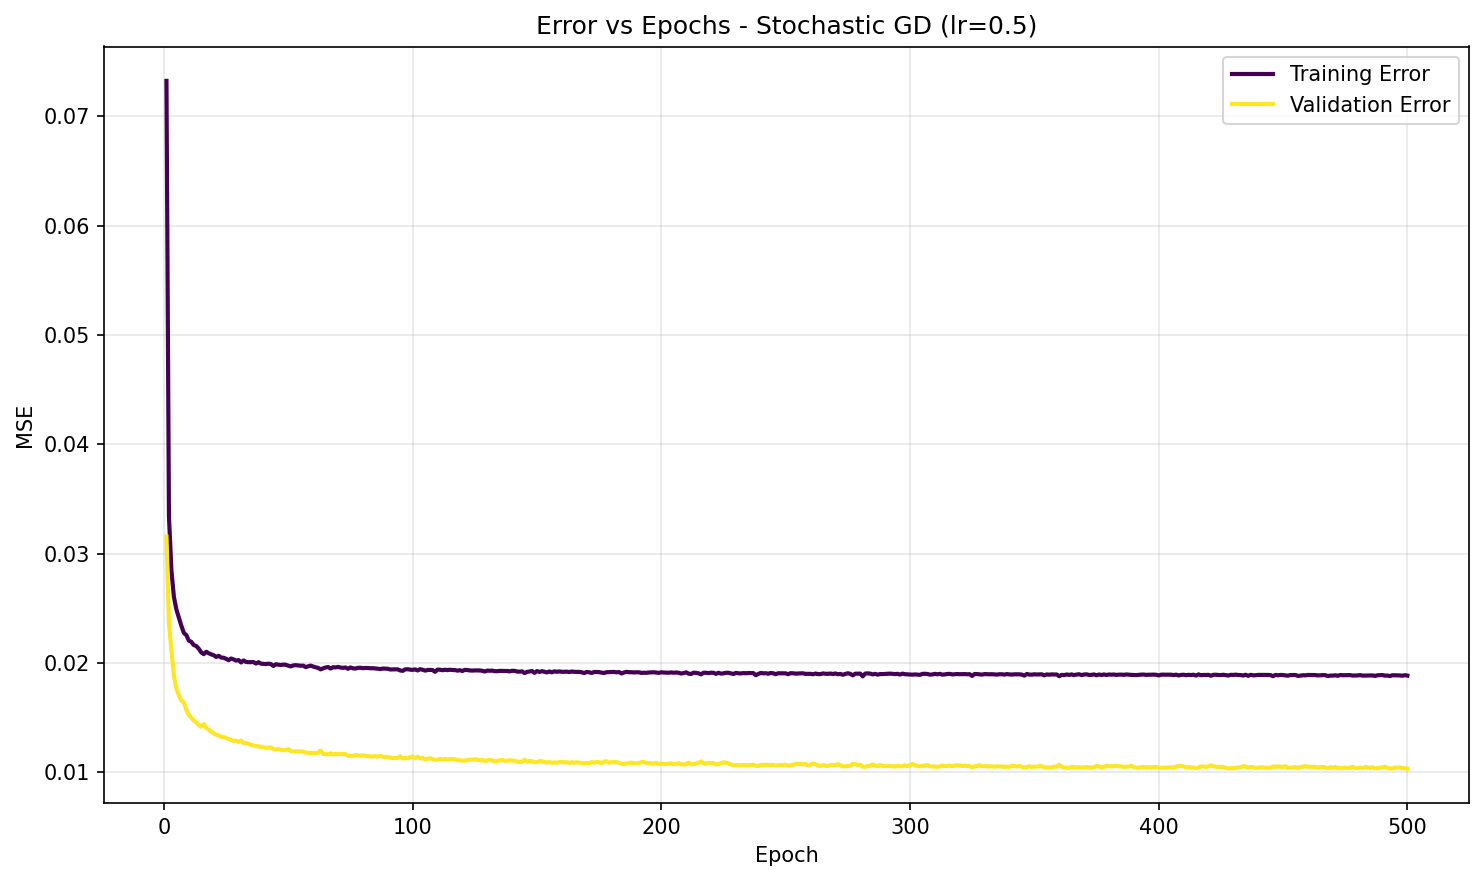
\includegraphics[width=0.85\linewidth]{2Lab/visualizations/error_sgd.png}
    \caption{Paklaidos priklausomybė nuo epochų (stochastinis GN, $\eta = 0{,}5$)}
    \label{fig:error_sgd}
\end{figure}
\subsection{Klasifikavimo tikslumo priklausomybė nuo epochų}
\label{subsec:tikslumas_nuo_epochu}

Šiame poskyryje aptariama klasifikavimo tikslumo priklausomybė nuo epochų abiems taikytiems metodams.

\subsubsection{Paketinis gradientinis nusileidimas}
\label{subsubsec:klasifikavimo_tikslumas_paketinis_gradientinis_nusileidimas}

Klasifikavimo tikslumas sparčiai auga pirmųjų epochų metu ir stabilizuojasi apie $97\ \%$ mokymo duomenims bei $98{,}2\ \%$ validavimo duomenims (žr.~\ref{fig:accuracy_bgd} pav.).

\begin{figure}[H]
    \centering
    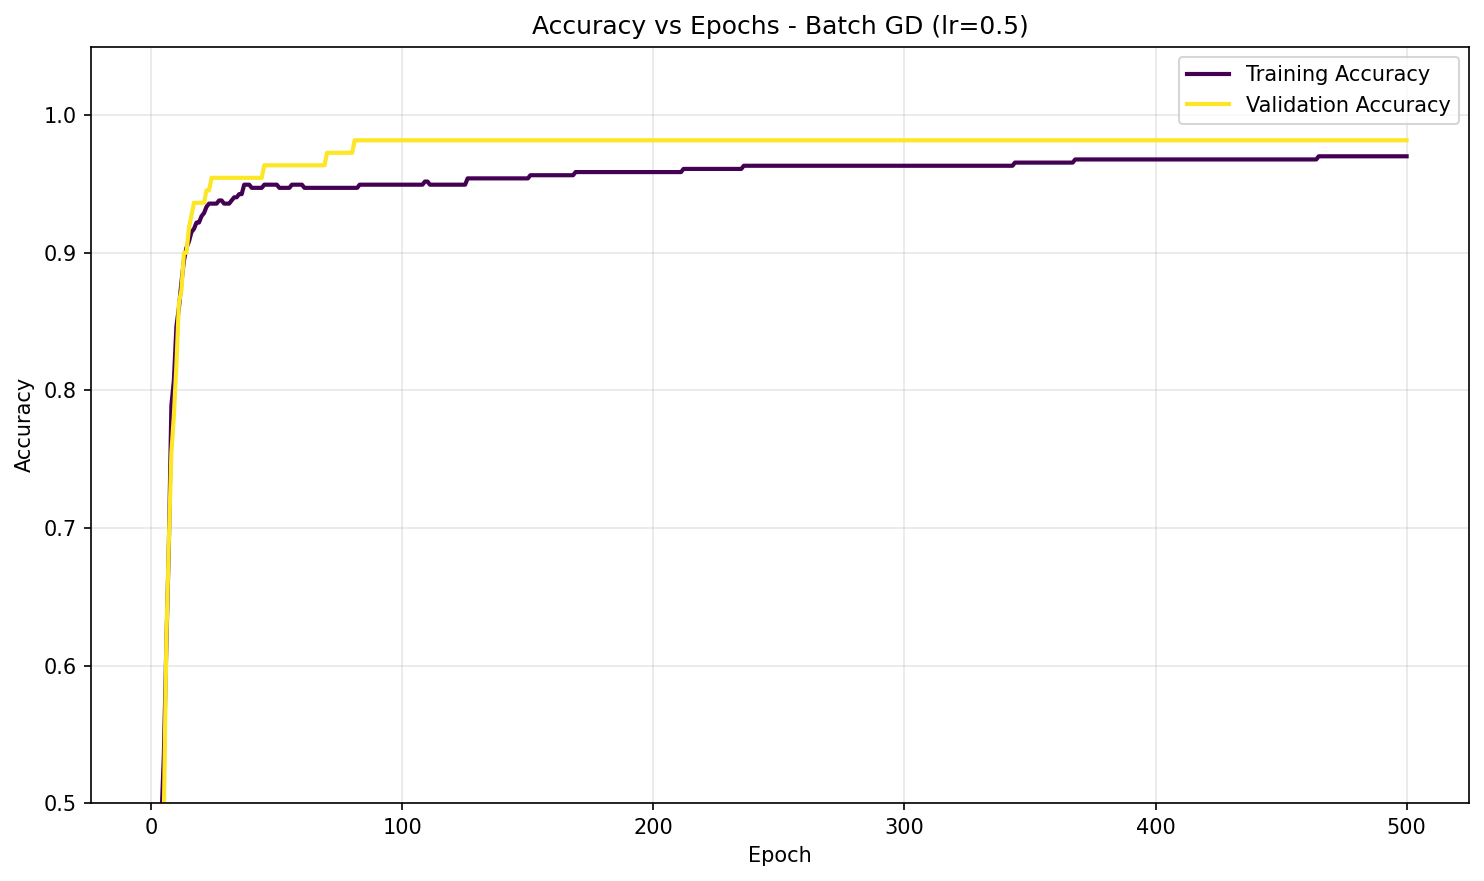
\includegraphics[width=0.85\linewidth]{2Lab/visualizations/accuracy_bgd.png}
    \caption{Klasifikavimo tikslumo priklausomybė nuo epochų (paketinis GN, $\eta = 0{,}5$)}
    \label{fig:accuracy_bgd}
\end{figure}
\subsubsection{Stochastinis gradientinis nusileidimas}
\label{subsubsec:klasifikavimo_tikslumas_stochastinis_gradientinis_nusileidimas}

Stochastinio metodo tikslumas taip pat greitai auga ir pasiekia $97{,}9\ \%$ mokymo duomenims bei $99{,}1\ \%$ validavimo duomenims (žr.~\ref{fig:accuracy_sgd} pav.). Validavimo tikslumas yra aukštesnis nei paketinio metodo atveju.

\begin{figure}[H]
    \centering
    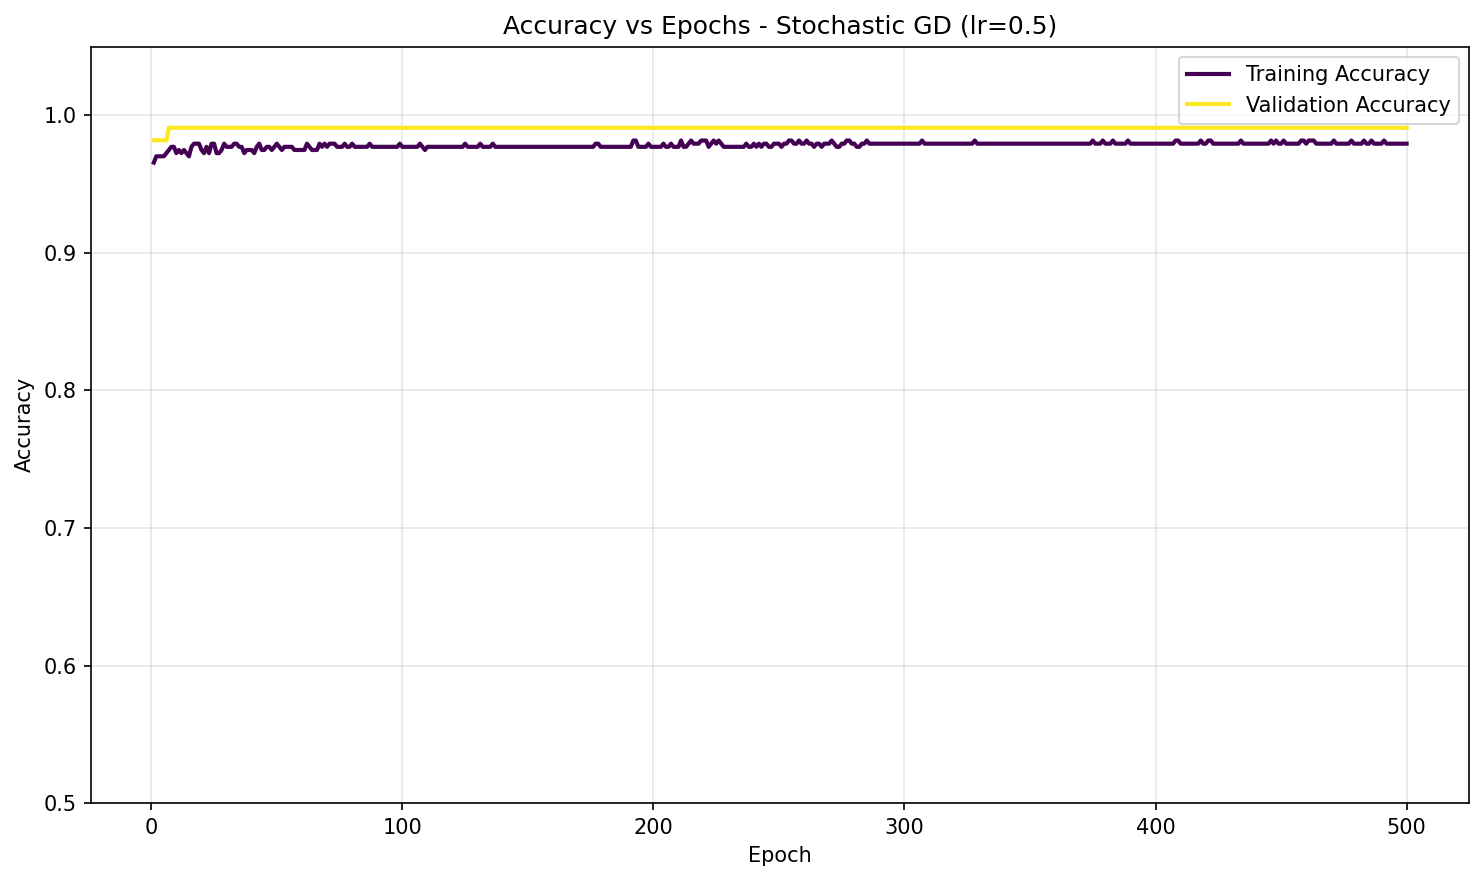
\includegraphics[width=0.85\linewidth]{2Lab/visualizations/accuracy_sgd.png}
    \caption{Klasifikavimo tikslumo priklausomybė nuo epochų (stochastinis GN, $\eta = 0{,}5$)}
    \label{fig:accuracy_sgd}
\end{figure}
\subsection{Mokymosi greičio įtaka rezultatams}
\label{subsec:mokymosi_greicio_itaka}

Buvo ištirtos keturios mokymosi greičio reikšmės: $0{,}01$, $0{,}1$, $0{,}5$ ir $0{,}9$. Rezultatai pateikti~\ref{tab:lr_comparison} lentelėje.

\begin{table}[H]
    \centering
    \caption{Mokymosi greičio įtaka validavimo tikslumui ($500$ epochų).}
    \begin{tabular}{|c|c|c|}
        \hline
        $\eta$ & BGN validavimo tikslumas & SGN validavimo tikslumas \\
        \hline
        $0{,}01$ & $81{,}8\ \%$ & $99{,}1\ \%$ \\ \hline
        $0{,}1$ & $98{,}2\%$ & $99{,}1\ \%$ \\ \hline
        $0{,}5$ & $98{,}2\ \%$ & $99{,}1\ \%$ \\ \hline
        $0{,}9$ & $98{,}2\ \%$ & $99{,}1\ \%$ \\ \hline
    \end{tabular}
    \label{tab:lr_comparison}
\end{table}

Paketinis gradientinis nusileidimas yra jautresnis mokymosi greičio parinkimui – su $\eta = 0{,}01$ validavimo tikslumas siekia tik $81{,}8\ \%$, nes per $500$ epochų modelis nespėja pakankamai konverguoti. Didinant $\eta$ iki $0{,}1$ ir daugiau, tikslumas stabilizuojasi ties $98{,}2\ \%$ (žr.~\ref{fig:lr_comparison_bgd} pav.).

Stochastinis gradientinis nusileidimas yra atsparesnis mokymosi greičio pasirinkimui – visais keturiais atvejais pasiekiamas $99{,}1\ \%$ validavimo tikslumas (žr.~\ref{fig:lr_comparison_sgd} pav.).

\begin{figure}[H]
    \centering
    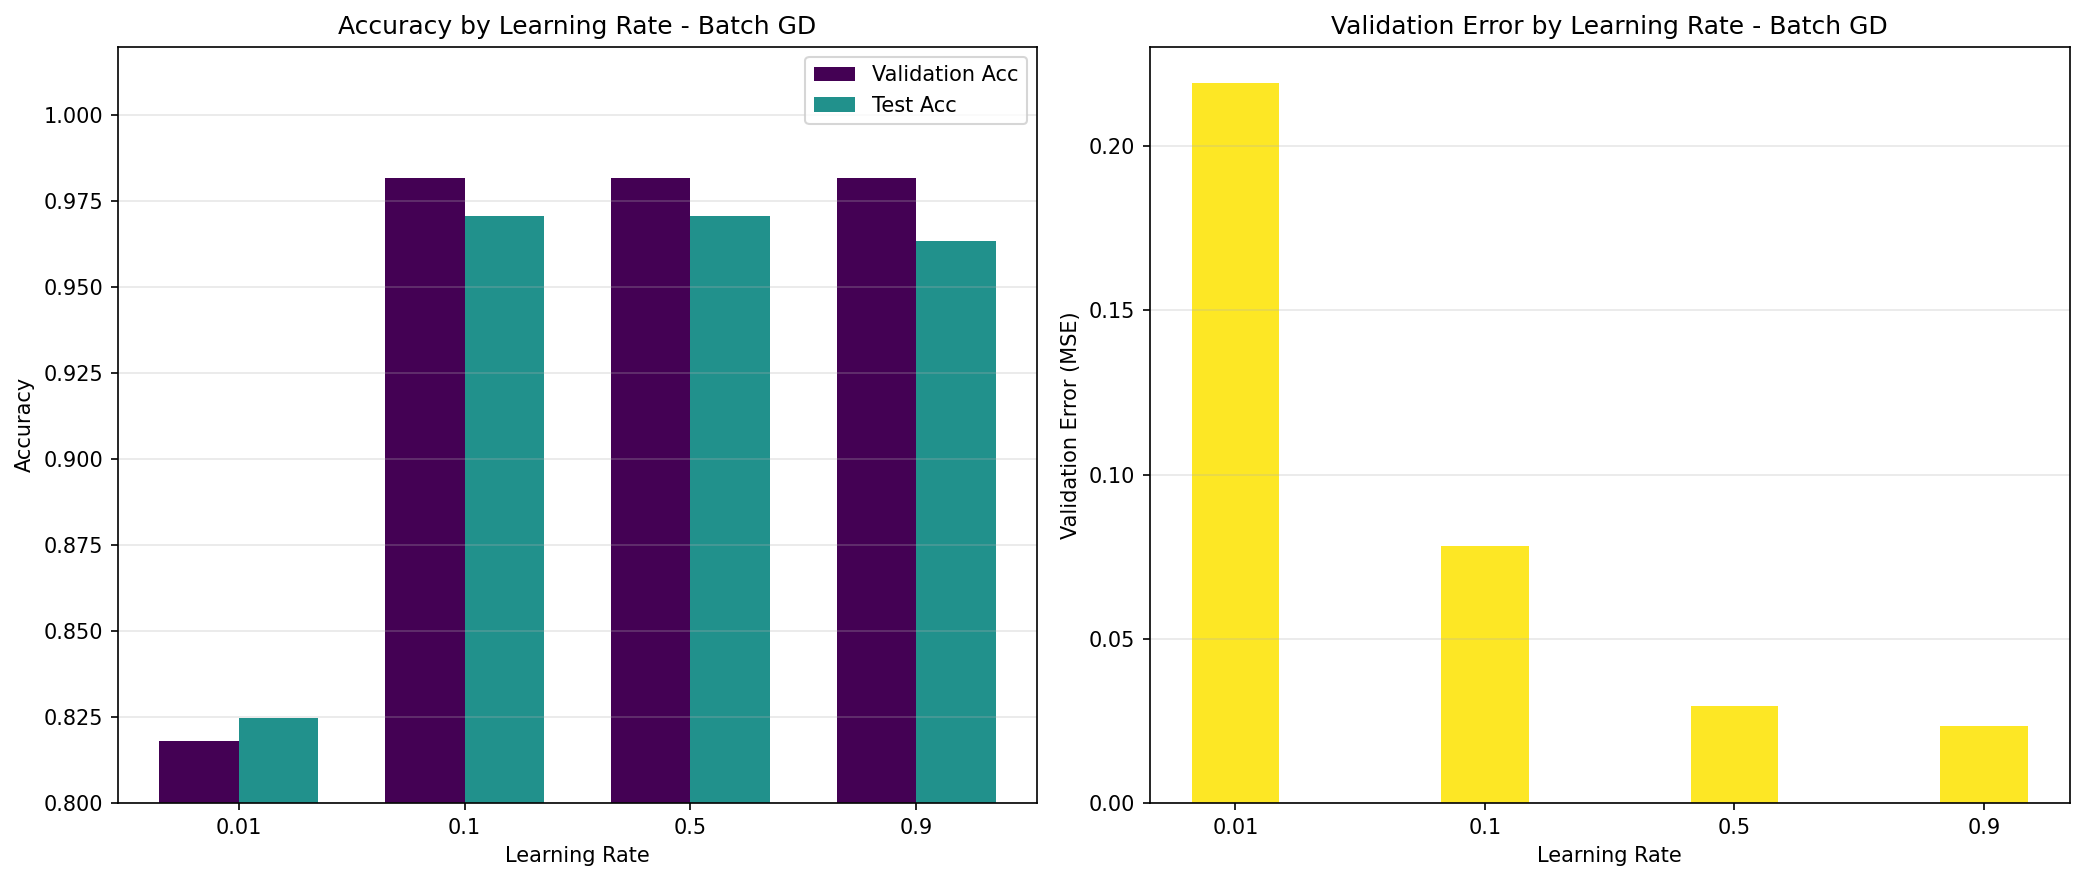
\includegraphics[width=0.85\linewidth]{2Lab/visualizations/lr_comparison_bgd.png}
    \caption{Mokymosi greičio įtaka rezultatams (paketinis GN)}
    \label{fig:lr_comparison_bgd}
\end{figure}

\begin{figure}[H]
    \centering
    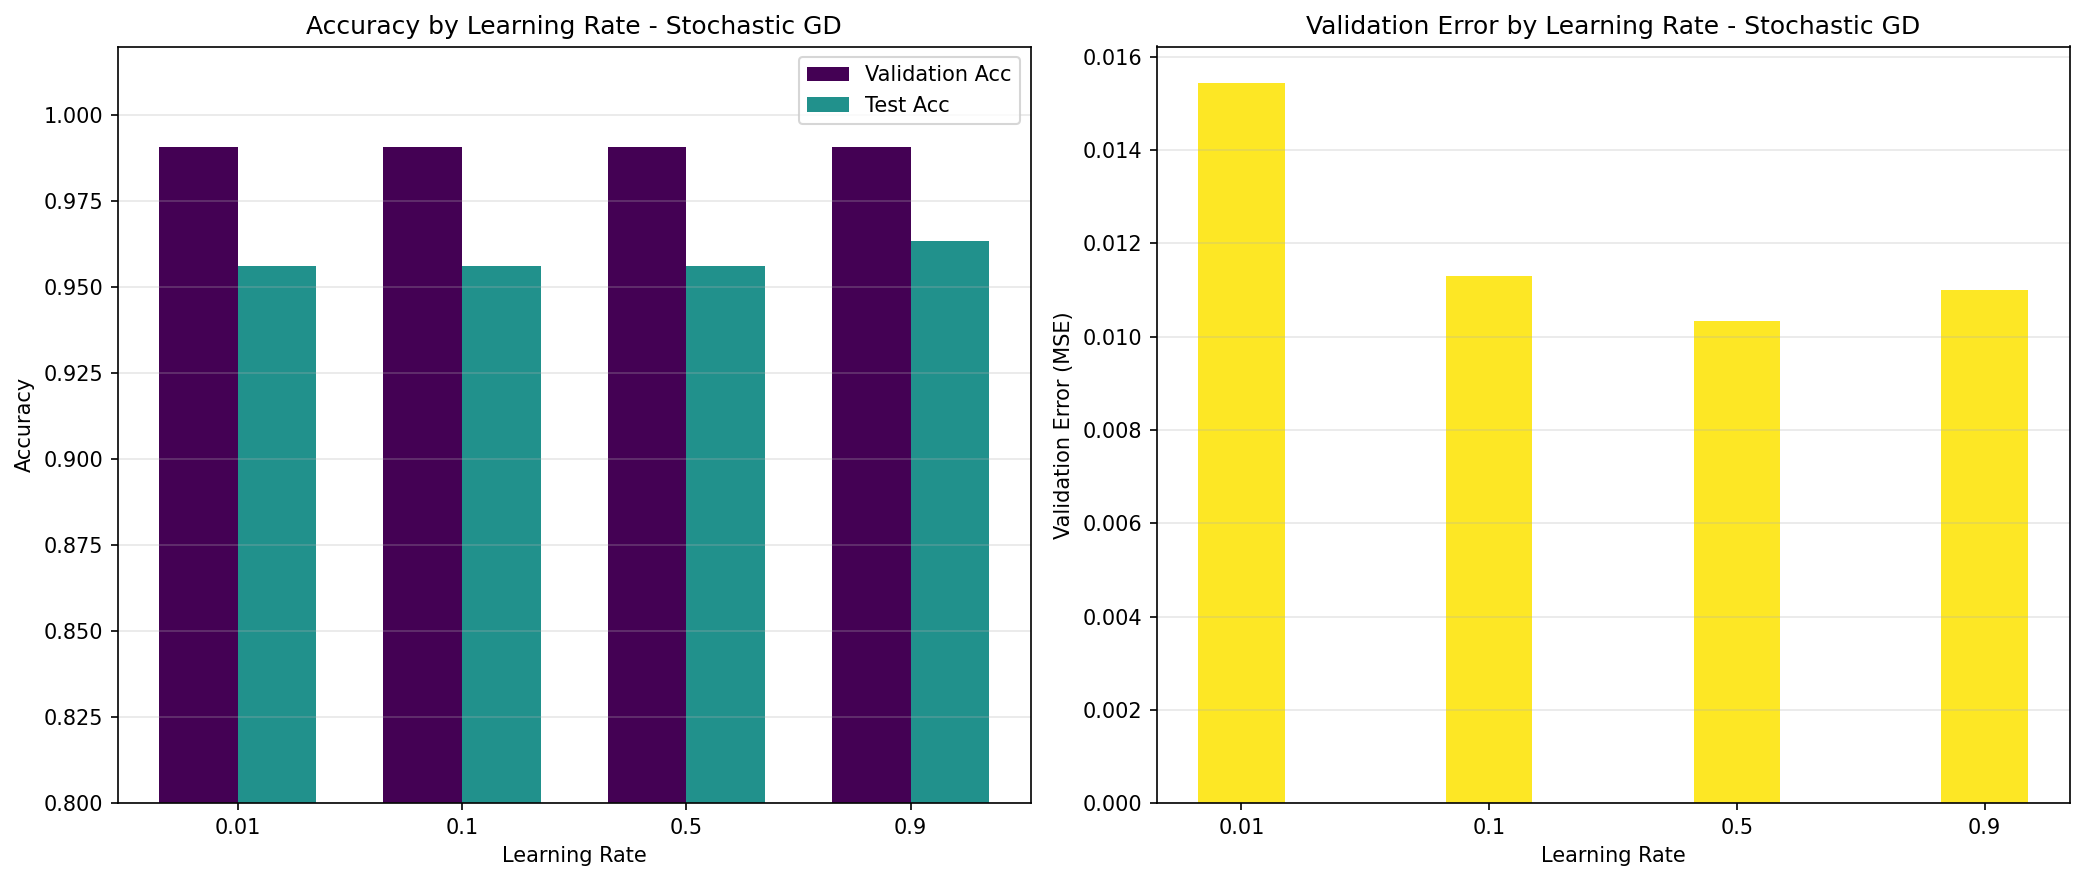
\includegraphics[width=0.85\linewidth]{2Lab/visualizations/lr_comparison_sgd.png}
    \caption{Mokymosi greičio įtaka rezultatams (stochastinis GN)}
    \label{fig:lr_comparison_sgd}
\end{figure}
\subsection{Paketinio ir stochastinio gradientinio nusileidimo palyginimas}
\label{subsec:bgd_vs_sgd}

Šiame poskyryje palyginami paketinio ir gradientinio nusileidimo metodai.

\subsubsection{Paklaida ir tikslumas}

Abiejų metodų paklaidos ir tikslumo kreivės palygintos~\ref{fig:bgd_vs_sgd_error} ir~\ref{fig:bgd_vs_sgd_accuracy} paveiksluose.

\begin{figure}[H]
    \centering
    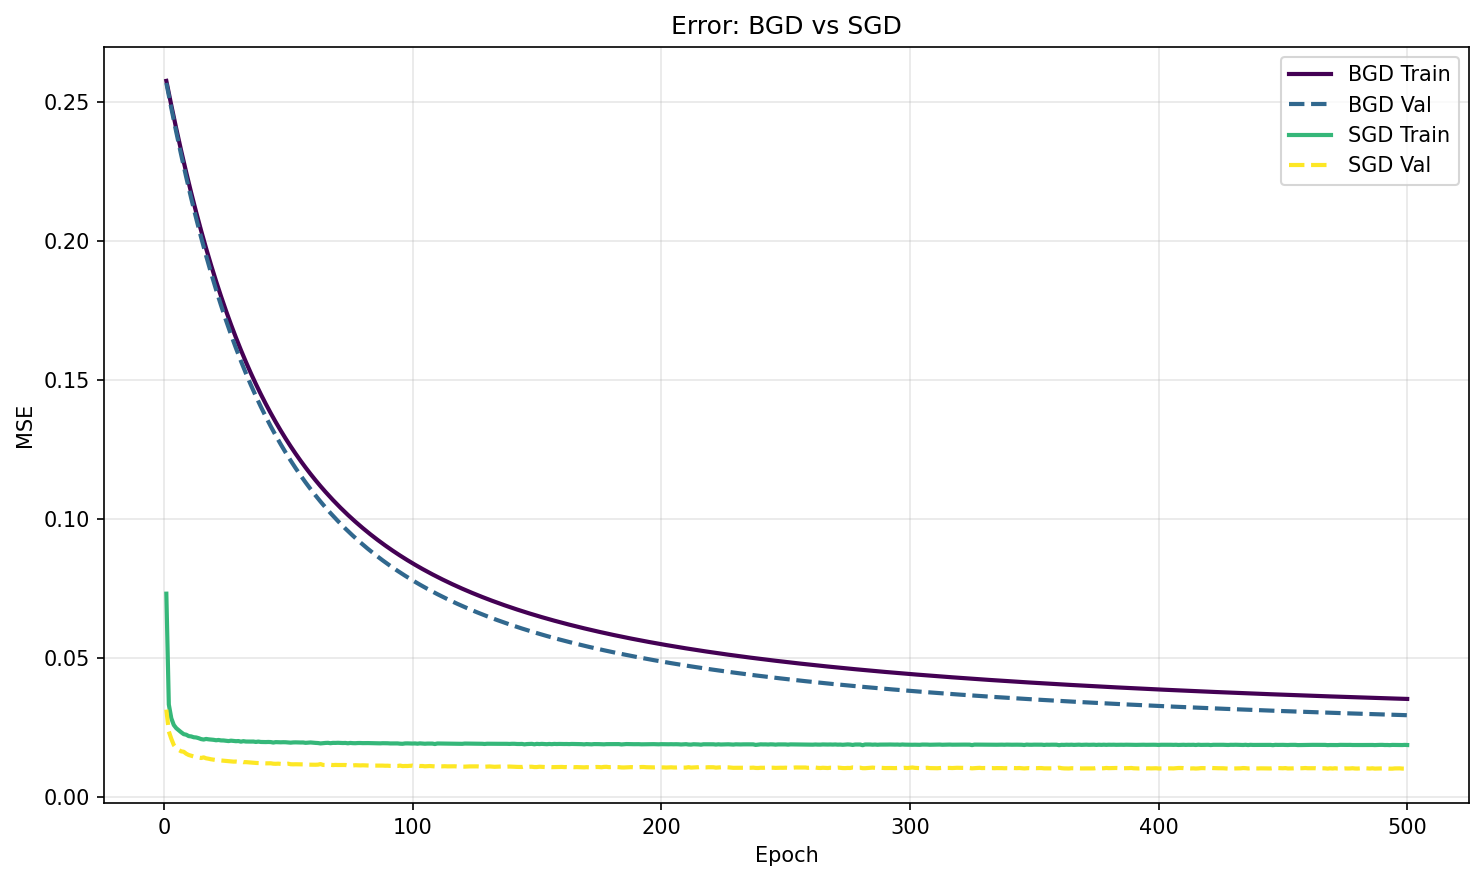
\includegraphics[width=0.85\linewidth]{2Lab/visualizations/bgd_vs_sgd_error.png}
    \caption{Paklaidos palyginimas: paketinis ir stochastinis GN}
    \label{fig:bgd_vs_sgd_error}
\end{figure}

\begin{figure}[H]
    \centering
    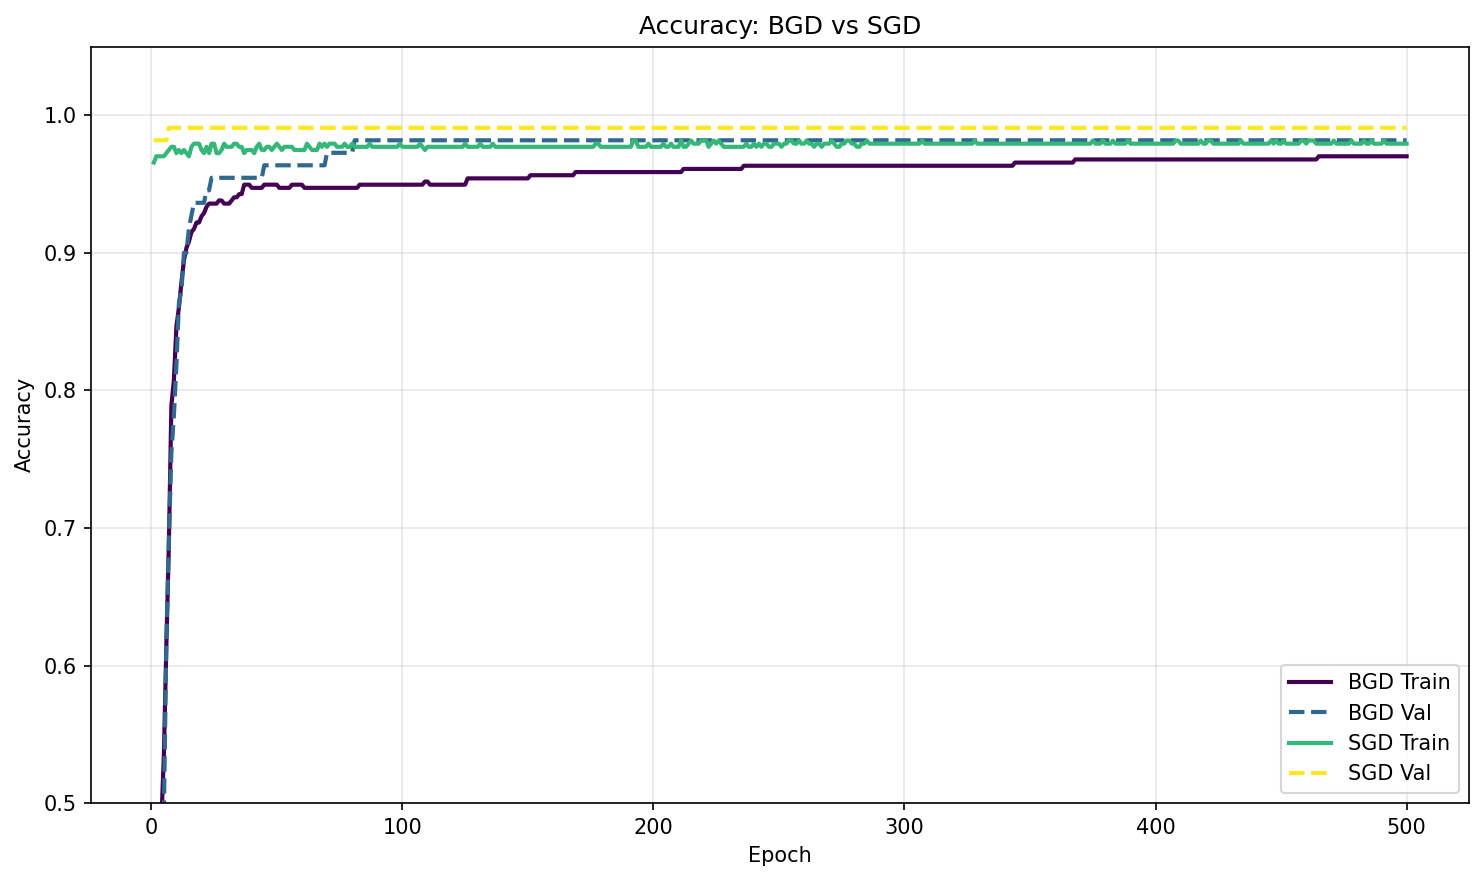
\includegraphics[width=0.85\linewidth]{2Lab/visualizations/bgd_vs_sgd_accuracy.png}
    \caption{Tikslumo palyginimas: paketinis ir stochastinis GN}
    \label{fig:bgd_vs_sgd_accuracy}
\end{figure}

Stochastinis gradientinis nusileidimas pasiekia mažesnę paklaidą ir aukštesnį validavimo tikslumą ($99{,}1\ \%$) nei paketinis ($98{,}2\ \%$). Tačiau testavimo duomenims paketinis metodas pasiekia aukštesnį tikslumą ($97{,}1\ \%$) nei stochastinis ($95{,}6\ \%$), o tai rodo, kad stochastinis metodas gali šiek tiek persimokyti validavimo duomenims (žr.~\ref{fig:bgd_vs_sgd_val_accuracy} pav.).

\begin{figure}[H]
    \centering
    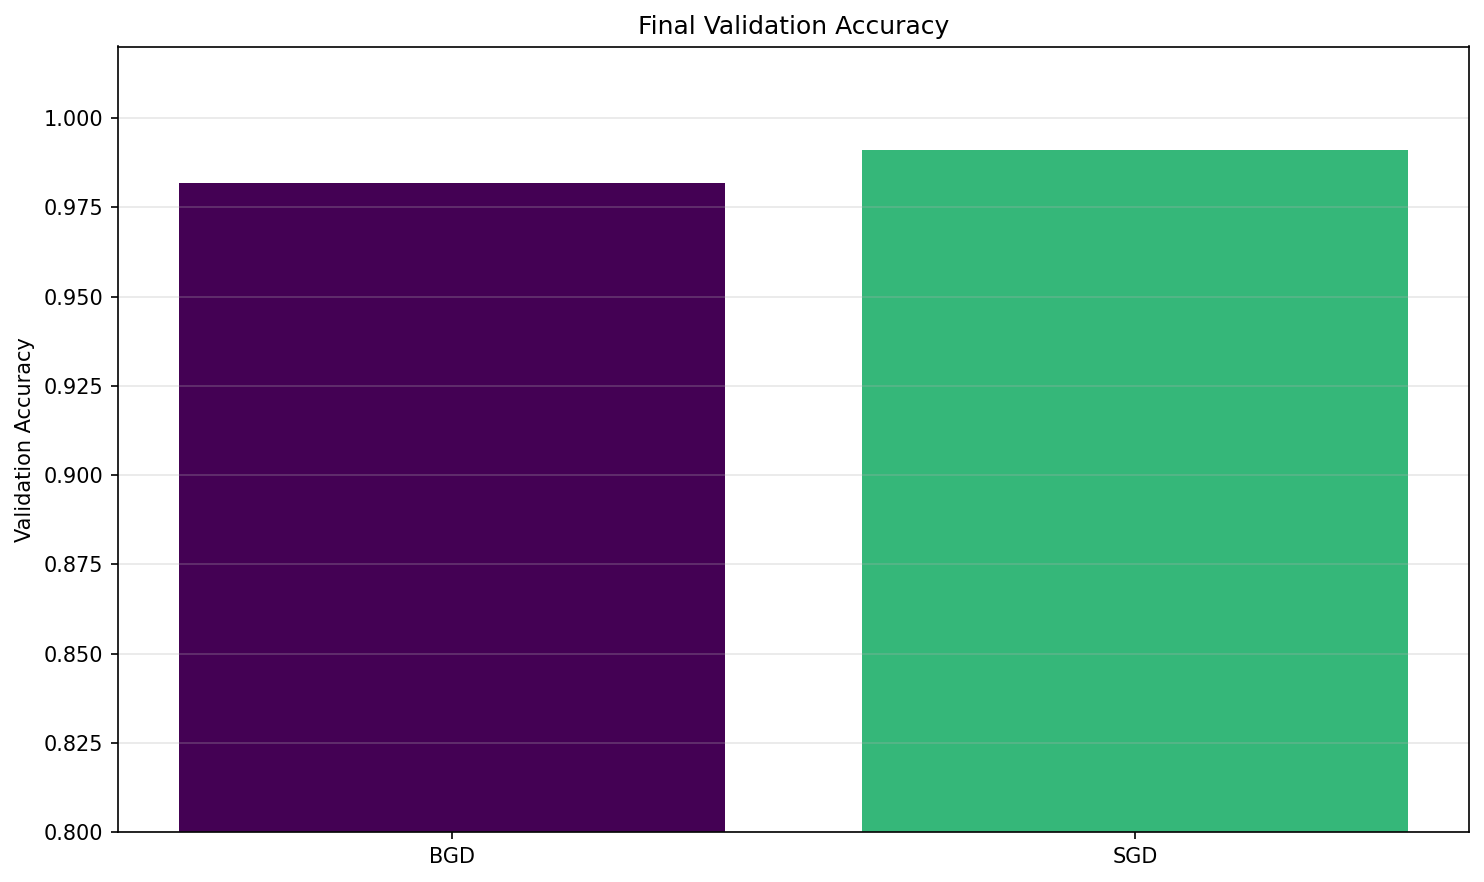
\includegraphics[width=0.85\linewidth]{2Lab/visualizations/bgd_vs_sgd_val_accuracy.png}
    \caption{Galutinis validavimo tikslumas: paketinis ir stochastinis GN}
    \label{fig:bgd_vs_sgd_val_accuracy}
\end{figure}
\subsubsection{Mokymo laiko palyginimas}

Mokymo laikas buvo palygintas esant vienodam epochų skaičiui ($100$, $300$, $500$). Rezultatai pateikti~\ref{tab:time_comparison} lentelėje ir~\ref{fig:time_comparison} paveiksle.

\begin{table}[H]
    \centering
    \caption{Mokymo laiko palyginimas (sekundėmis).}
    \begin{tabular}{|c|c|c|}
        \hline
        Epochų skaičius & Paketinis GN & Stochastinis GN \\
        \hline
        $100$ & $0{,}45$ s & $0{,}45$ s \\ \hline
        $300$ & $1{,}39$ s & $1{,}57$ s \\ \hline
        $500$ & $3{,}05$ s & $3{,}36$ s \\ \hline
    \end{tabular}
    \label{tab:time_comparison}
\end{table}

\begin{figure}[H]
    \centering
    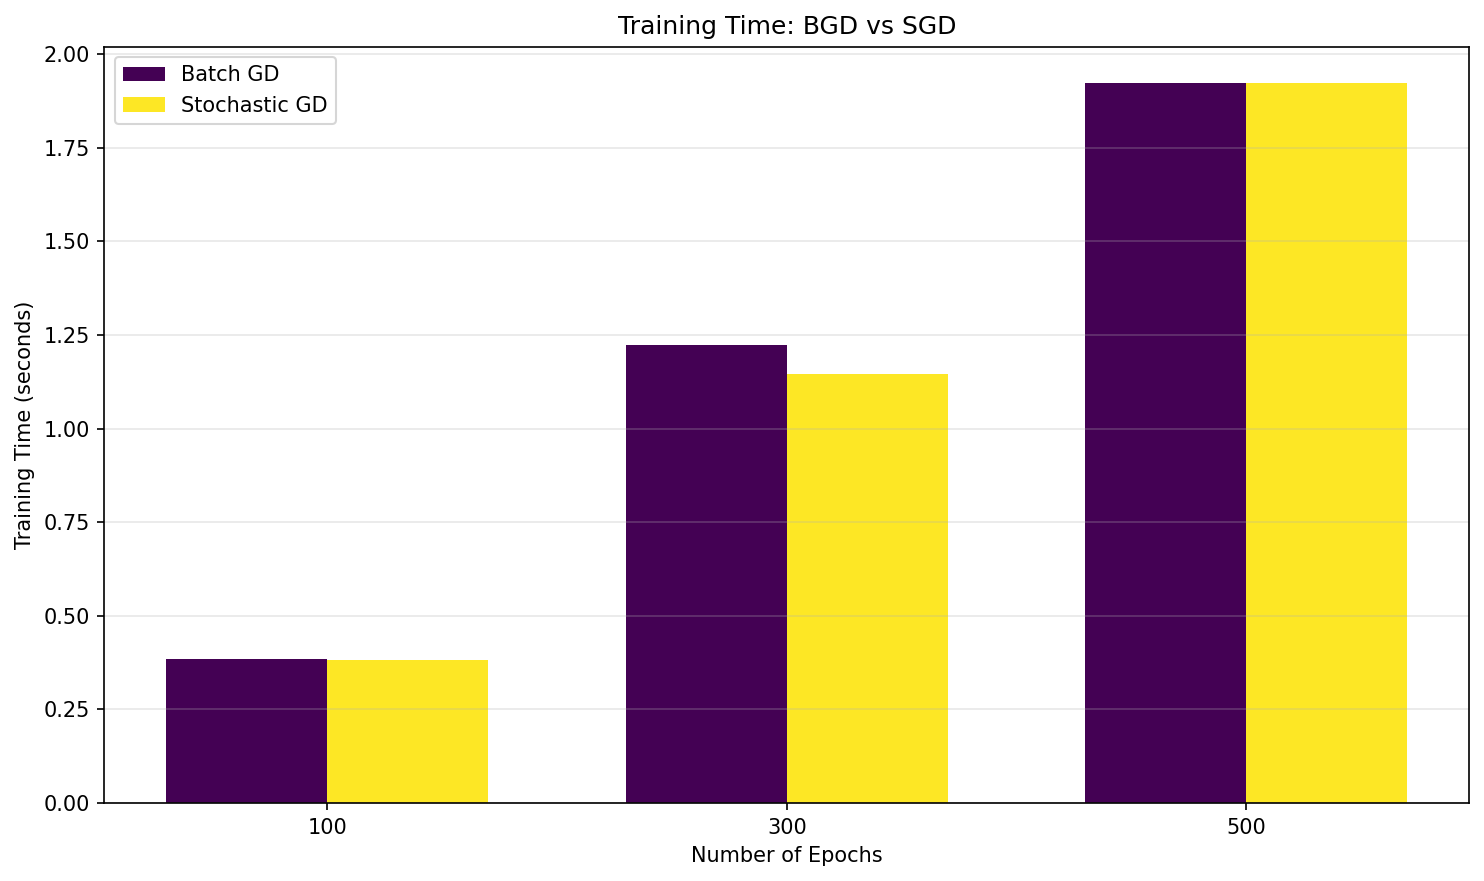
\includegraphics[width=0.85\linewidth]{2Lab/visualizations/time_comparison.png}
    \caption{Mokymo laiko palyginimas esant vienodam epochų skaičiui}
    \label{fig:time_comparison}
\end{figure}

Mokymo laikas abiem metodams yra panašus išskyrus atvejį su $epoch = 500$. Didėjant epochų skaičiui pradeda matytis, jog stochastinis metodas tampa greitesniu, tačiau skirtumas nėra didelis.